\section{Cornering Model}
\label{sec:cornering-model}

Whenever the track's curvature profile $\kappa(s)$ (\cref{sec:track-geometry})
is nonzero, the simulation adds a lean-angle and banked-rolling-resistance
correction to the equation of motion (\cref{sec:lean-angle,sec:rolling-resistance}).
If the rider's center-of-mass height $h$ (\nolinkurl{com_height_m}) is also
known, two further corrections activate: the wheel-speed geometric correction
and the corner component of acceleration
(\cref{sec:wheel-speed-geometry,sec:energy-feedback}). This section derives
each term in turn.

\subsection{Framing: quasi-static lean angle}
\label{sec:quasi-static-lean}

The lean angle $\theta$ derived below is easy to over-read as a full rigid-body
treatment; it is not one. $\theta$ is \emph{algebraically constrained} to
the instantaneous speed $v$ and track curvature $\kappa$ at every instant; it is
not an independent state variable with its own rotational inertia, and the model
does not track a separate roll rate. There is also no friction-circle or
traction-limit check: $\theta$ is computed unconditionally from $v$ and
$\kappa$ regardless of whether the tire could actually supply the implied
lateral friction. This is a deliberate simplification, revisited in
\cref{sec:assumptions}, appropriate for the smooth, moderate-curvature track
geometry of \cref{sec:track-geometry} but not a general-purpose vehicle dynamics
model.

\subsection{Lean angle}
\label{sec:lean-angle}

For a bicycle in a steady, flat turn of radius $r = 1/\kappa$ at speed $v$, the
classic no-slip lean-angle balance equates the lateral force required for
circular motion, $m v^2 / r$, with the horizontal component of gravity acting
through the lean:
\begin{equation}
    \tan\theta = \frac{v^2}{g r} = \frac{v^2 \kappa}{g}\ .
    \label{eq:lean-angle-tan}
\end{equation}
Solving for $\theta$,
\begin{equation}
    \theta(v,\kappa) = \arctan\!\left(\frac{v^2 \kappa}{g}\right)\ .
    \label{eq:lean-angle}
\end{equation}
On a straight ($\kappa = 0$) or at rest ($v=0$), $\theta = 0$ and every term
introduced in this section vanishes, so the model reduces exactly to
\cref{sec:simulation-model} with no cornering configured.

\subsection{Center-of-mass offset and wheel-speed geometry}
\label{sec:wheel-speed-geometry}

\begin{figure}[htbp]
    \centering
    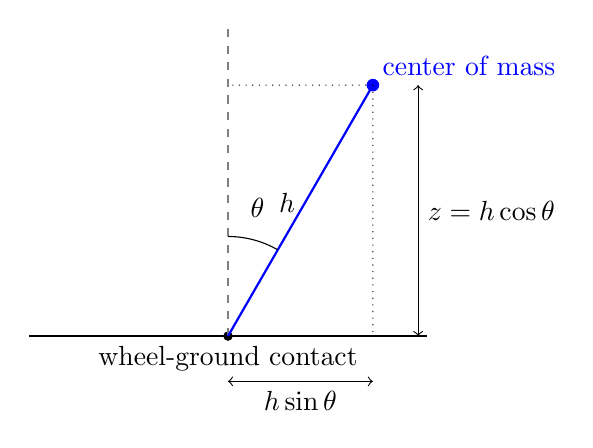
\begin{tikzpicture}[scale=1.15]
        \draw[thick] (-2.2,0) -- (2.2,0);
        \filldraw (0,0) circle (1.3pt);
        \node[below] at (0,0) {wheel-ground contact};
        \draw[dashed, gray] (0,0) -- (0,3.4);
        \draw[thick, blue] (0,0) -- (60:3.2) coordinate (com);
        \filldraw[blue] (com) circle (1.8pt);
        \node[above right, blue] at (com) {center of mass};
        \draw (0,1.1) arc (90:60:1.1);
        \node at (77:1.45) {$\theta$};
        \draw[dotted] (com) -- (0,{3.2*sin(60)});
        \draw[dotted] (com) -- ({3.2*cos(60)},0);
        \draw[<->] (0,-0.5) -- ({3.2*cos(60)},-0.5);
        \node[below] at ({0.5*3.2*cos(60)},-0.5) {$h\sin\theta$};
        \draw[<->] ({3.2*cos(60)+0.5},0) -- ({3.2*cos(60)+0.5},{3.2*sin(60)});
        \node[right] at ({3.2*cos(60)+0.5},{0.5*3.2*sin(60)}) {$z=h\cos\theta$};
        \node[left] at (60:1.7) {$h$};
    \end{tikzpicture}
    \caption{Lean geometry viewed from in front of the rider: the center of mass sits
    a distance $h$ from the wheel-ground contact point at lean angle $\theta$
    from vertical, with horizontal offset $h\sin\theta$ and height
    $z = h\cos\theta$ above the contact point.}
    \label{fig:lean-geometry}
\end{figure}

The state variable $v$ represents the speed of the rider's center of mass
(\cref{fig:lean-geometry}). When
leaned at angle $\theta$, the center of mass sits a horizontal distance
$h \sin\theta$ inboard of the wheel-ground contact line, tracing a smaller
effective turn radius than the wheels themselves, which remain on the racing
line. Writing $r = 1/\kappa$ for the wheels' turn radius, the center of mass
turns on a radius $r - h\sin\theta$. For the same angular sweep of the turn,
both the wheels and the center of mass sweep the same angle in the same time, so
their speeds scale directly with radius,
$v / v_{\mathrm{wheel}} = (r - h\sin\theta)/r = 1 - \kappa h \sin\theta$. Solving
for the wheel speed,
\begin{equation}
    v_{\mathrm{wheel}}(v, \kappa, \theta) =
        \frac{v}{1 - \kappa h \sin\theta}\ ,
    \label{eq:wheel-speed}
\end{equation}
with the denominator floored at $0.01$ in the implementation as a numerical
safeguard against extreme combinations of $\kappa$, $h$, and $\theta$ driving it
toward zero. This matters because track curvature $\kappa(s)$ is indexed by arc
length along the track surface -- the wheels' path -- not by the center of
mass's path. Consequently the position state advances at the wheel speed rather
than the center-of-mass speed,
\begin{equation}
    \frac{ds}{dt} = v_{\mathrm{wheel}}\ ,
    \label{eq:ds-dt}
\end{equation}
Equation \eqref{eq:ds-dt} itself only updates the position state; it is not a
term in $dv/dt$. The wheel speed $v_{\mathrm{wheel}}$ it defines, however, is
reused below in \cref{sec:energy-feedback}'s energy-feedback term, so the
cornering correction as a whole does still affect $dv/dt$, just not through
this equation.

Because the race-distance terminal event of \cref{sec:numerical-integration}
triggers when $s$ -- the same coordinate advanced via \cref{eq:ds-dt} --
reaches $s_{\mathrm{race}}$, the tracked race distance is a track-surface
(wheel-path) distance, matching how a race distance is physically marked on a
track. A direct consequence is that the rider's center of mass itself covers a
slightly shorter cumulative distance than $s_{\mathrm{race}}$ over the course
of a full run, since it cuts inside the wheels' path through every corner.

\subsection{Straight and corner components of acceleration}
\label{sec:accel-components}

The center of mass's total acceleration splits exactly into two additive
pieces: a straight-line piece, identical to what would apply on flat, straight
riding, and a cornering piece that appears only when the track curves.
Writing this decomposition for both $dv/dt$ and the scalar acceleration it
represents,
\begin{equation}
    \frac{dv}{dt} = \left(\frac{dv}{dt}\right)_{\text{straight}} + \left(\frac{dv}{dt}\right)_{\text{corner}}
    \qquad\text{equivalently}\qquad
    a = a_{\mathrm{straight}} + a_{\mathrm{corner}}\ .
    \label{eq:accel-split}
\end{equation}
The straight-line piece, $(dv/dt)_{\text{straight}} \equiv a_{\mathrm{straight}}$,
is exactly the non-cornering acceleration of \cref{eq:a-straight}: rolling
resistance, aerodynamic drag, and propulsive force, unaffected by lean. The
corner piece, $a_{\mathrm{corner}}$, is the acceleration contribution from the
rider leaning through the corner; the rest of this section derives it.

\subsection{Corner component of acceleration}
\label{sec:energy-feedback}

As the rider leans into and out of a corner, the center of mass moves
vertically. Defining $z \equiv h\cos\theta$ as the CoM height above the wheel path,
$z$ decreases as $\theta$ grows from zero -- leaning over lowers the
center of mass. By the conservation of energy, this loss of height converts
into a small \emph{gain} in forward speed on the way into a corner; the reverse
conversion, kinetic energy converting back into potential energy, gives a small
\emph{loss} of speed coming back upright on the way out. This subsection derives
that acceleration contribution, denoted $a_{\mathrm{corner}}$.

\subsubsection{Energy conservation on vertical CoM motion}

The center-of-mass height above a fixed reference is, up to a constant,
$h\cos\theta$, so its vertical velocity is
$\frac{dz}{dt} = -h\sin\theta\,\frac{d\theta}{dt}$. Energy conservation on the
combined kinetic and potential terms, $\frac{d}{dt}\!\left(\tfrac{1}{2}v^2 + gz\right) = 0$
for the lean-driven exchange alone, gives
$v\,(dv/dt)_{\text{corner}} = gh\sin\theta\,\frac{d\theta}{dt}$,
or
\begin{equation}
    a_{\mathrm{corner}} = \frac{gh\sin\theta}{v}\,\frac{d\theta}{dt}\ .
    \label{eq:a-corner-general}
\end{equation}

\subsubsection{Chain-rule decomposition: the (s) and (v) parts}

$\theta$ depends on both position and speed, $\theta(v,\kappa(s))$, so by the
chain rule,
\begin{equation}
    \frac{d\theta}{dt} =
        \underbrace{\left.\frac{\partial\theta}{\partial s}\right|_v \frac{ds}{dt}}_{\text{driven by moving through the corner}}
        \;+\;
        \underbrace{\frac{\partial\theta}{\partial v}\,\frac{dv}{dt}}_{\text{driven by }v\text{ itself changing}}\ .
    \label{eq:dtheta-dt-chain-rule}
\end{equation}
Substituting into \cref{eq:a-corner-general} splits $a_{\mathrm{corner}}$ into
two additive contributions, named for the chain-rule term that produced them:
\begin{equation}
    a_{\mathrm{corner}} = a_{\mathrm{corner}}^{(s)} + a_{\mathrm{corner}}^{(v)}\ ,
    \qquad
    a_{\mathrm{corner}}^{(s)} \equiv
        \frac{gh\sin\theta}{v}\left.\frac{\partial\theta}{\partial s}\right|_v\frac{ds}{dt}\ ,
    \qquad
    a_{\mathrm{corner}}^{(v)} \equiv
        \frac{gh\sin\theta}{v}\frac{\partial\theta}{\partial v}\,\frac{dv}{dt}\ .
    \label{eq:a-corner-split}
\end{equation}
$a_{\mathrm{corner}}^{(s)}$ depends only on quantities already known from the
current state ($v$, $s$, and quantities derived from them); it can be computed
directly, the same way $a_{\mathrm{straight}}$ can. $a_{\mathrm{corner}}^{(v)}$,
by contrast, depends on $dv/dt$ itself -- the \emph{total} derivative being
solved for, not just the corner piece of it -- since $\theta$'s dependence on
$v$ feeds back into the very acceleration being computed. Left in this form,
the equation of motion would have $dv/dt$ appearing on both sides; the next
two subsubsections derive $\partial\theta/\partial s|_v$ and
$\partial\theta/\partial v$ explicitly, after which
\cref{sec:combined-eom} rearranges and solves for $dv/dt$.

\subsubsection{Explicit s-dependence of theta}

Differentiating \cref{eq:lean-angle-tan} implicitly with respect to arc length
$s$ at fixed $v$, using $\frac{d}{ds}\tan\theta = \sec^2\theta\,
\partial\theta/\partial s$ and the identity $\sec^2\theta = 1+\tan^2\theta$,
gives
\begin{equation}
    \sec^2\theta\left.\frac{\partial\theta}{\partial s}\right|_{v} =
        \frac{v^2}{g}\,\frac{d\kappa}{ds}
    \quad\Longrightarrow\quad
    \left.\frac{\partial\theta}{\partial s}\right|_{v} =
        \cos^2\theta\,\frac{v^2}{g}\,\frac{d\kappa}{ds}\ ,
    \label{eq:dtheta-ds}
\end{equation}
the rate of change of lean angle due to the changing curvature alone. This
derivative is well-defined everywhere: \cref{sec:curvature-smoothing} constructs
$\kappa(s)$ as a smoothed, differentiable profile rather than a step function,
so $d\kappa/ds$ is a genuine, bounded function of $s$ rather than a delta spike
at each corner boundary. (The implementation computes this equivalent form as
$1/(1+x^2)$ with
$x \equiv \tan\theta = v^2\kappa/g$, identical to $\cos^2\theta$ by the same
identity.)

The other factor needed for $a_{\mathrm{corner}}^{(s)}$, $ds/dt$, is already
established: it is exactly the wheel speed $v_{\mathrm{wheel}}$ of
\cref{eq:ds-dt} from \cref{sec:wheel-speed-geometry}, so no further derivation
is needed here. Substituting both into \cref{eq:a-corner-split} makes
$a_{\mathrm{corner}}^{(s)}$ fully explicit:
\begin{equation}
    a_{\mathrm{corner}}^{(s)} =
        \frac{gh\sin\theta}{v}\left(\frac{\partial\theta}{\partial s}\right)v_{\mathrm{wheel}}\ .
    \label{eq:a-corner-s}
\end{equation}

\subsubsection{Implicit v-dependence of theta and the feedback coefficient}

Differentiating \cref{eq:lean-angle-tan} implicitly with respect to $v$ at
fixed $\kappa$ the same way gives the remaining, $v$-driven factor:
\begin{equation}
    \frac{\partial\theta}{\partial v} =
        \cos^2\theta\,\frac{2v\kappa}{g}\ .
    \label{eq:dtheta-dv}
\end{equation}
Substituting into \cref{eq:a-corner-split} makes $a_{\mathrm{corner}}^{(v)}$
explicit as well:
\begin{equation}
    a_{\mathrm{corner}}^{(v)} =
        \frac{gh\sin\theta}{v}\left(\frac{\partial\theta}{\partial v}\right)\frac{dv}{dt}
        = C(v,\kappa,\theta,h)\cdot\frac{dv}{dt}\ ,
    \label{eq:a-corner-v}
\end{equation}
where every explicit factor of $v$ and $g$ introduced by the
$gh\sin\theta/v$ prefactor of \cref{eq:a-corner-general} and the $2v\kappa/g$
factor of \cref{eq:dtheta-dv} cancels, leaving
\begin{equation}
    C(v,\kappa,\theta,h) =
        2 h \kappa \sin\theta \cos^2\theta\ ,
    \label{eq:feedback-coeff}
\end{equation}
independent of both $v$ and $g$. Substituting \cref{eq:a-corner-v} into
\cref{eq:a-corner-split} and adding the result to the straight-line
acceleration of \cref{eq:accel-split} gives the full equation of motion in the
form
\begin{equation}
    \frac{dv}{dt} = a_{\mathrm{straight}} + a_{\mathrm{corner}}^{(s)} +
        C(v,\kappa,\theta,h) \cdot \frac{dv}{dt}\ ,
    \label{eq:dv-dt-implicit}
\end{equation}
self-referential in $dv/dt$ through $\theta$'s own dependence on $v$.

\subsection{Combined equation of motion}
\label{sec:combined-eom}

Because $C$ enters \cref{eq:dv-dt-implicit} linearly, $dv/dt$ can be solved for
explicitly rather than treated as a second implicit unknown requiring its own
root-find at every solver step. Solving \cref{eq:dv-dt-implicit} for $dv/dt$
gives the full cornering-corrected equation of motion:
\begin{equation}
    \frac{dv}{dt} =
        \frac{a_{\mathrm{straight}} + a_{\mathrm{corner}}^{(s)}}
             {\max\bigl(1 - C,\ 0.1\bigr)}\ .
    \label{eq:dv-dt-full}
\end{equation}
The floor on the denominator is a numerical safeguard against $C$ approaching
$1$, which would only occur at combinations of lean, curvature, and speed far
outside any realistic riding condition; it has no physical interpretation. Together
with \cref{eq:ds-dt}, \cref{eq:dv-dt-full} completes the right-hand side of the
ODE integrated in \cref{sec:numerical-integration}.

As a consistency check, this construction is antisymmetric between corner entry
and corner exit: because $d\kappa/ds$ changes sign between the entry and exit
transition ramps of \cref{sec:track-geometry} while $v$ and $\theta$ are
approximately unchanged, $a_{\mathrm{corner}}^{(s)}$ takes equal and opposite
values entering and exiting a corner at the same speed. Over a full lean-in and
lean-out cycle at constant $v$, the term therefore integrates to zero net effect
on speed, consistent with energy conservation.

\subsection{Low-speed floor}
\label{sec:v-eps}

The corner-acceleration terms of this section -- $a_{\mathrm{corner}}$ and the
feedback coefficient $C$ -- are set to zero whenever $v < V_{\mathrm{eps}}$
(\SI{0.1}{\metre\per\second}). This avoids division-by-near-zero in
\cref{eq:a-corner-general}, the only one of the two with an explicit $1/v$
term; \cref{eq:feedback-coeff} has no such term (it depends only on $\kappa$,
$h$, and $\theta$) but is zeroed alongside it for consistency, since both
represent the same near-zero-speed cornering-energy exchange. (Lean angle
$\theta$ and the banked rolling resistance of \cref{sec:rolling-resistance} are
not gated this way; both remain well-defined at $v = 0$, where $\theta \to 0$
smoothly.) This is a numerical safeguard for the simulation's start condition,
not a distinct physical regime.
